%
% hardware.tex
%
% Copyright (C) 2020 by SpaceLab.
%
% PC-104 Adapter Documentation
%
% This work is licensed under the Creative Commons Attribution-ShareAlike 4.0
% International License. To view a copy of this license,
% visit http://creativecommons.org/licenses/by-sa/4.0/.
%

%
% \brief Hardware overview chapter.
%
% \author Gabriel Mariano Marcelino <gabriel.mm8@gmail.com>
%
% \institution Universidade Federal de Santa Catarina (UFSC)
%
% \version 2.0.0
%
% \date 2020/09/25
%

\chapter{Hardware Overview} \label{ch:hardware}

The hardware project is composed by two boards: top and bottom. Both PCB\nomenclature{\textbf{PCB}}{\textit{Printed Circuit Board.}}s were designed using KiCad v5.1.8-5 \cite{kicad}. Both boards also have the same size, shape and number of layers (4), and are vertically symmetrical (same components, but in different sides of the board).

All pins of the PC-104 connector are routed between the two boards, this way, this adapter can be used in any configuration of the PC-104 pins.

Both boards also have an inner cavity to allow vertically passing internal cables of the satellite. All the screw holes are connected to the copper planes of the board, but isolated from the PC-104 tracks (in other words, no signal is grounded to the chassi).

\section{Top Board}

The top board is composed by eight PicoBlade connectors (13 pins, straight, male) and a female PC-104 connector. A 3D model of the top board can be seen in Figures \ref{fig:top-board-top} (top side) and \ref{fig:top-board-bottom} (bottom side).

\begin{figure}[!htb]
    \begin{center}
        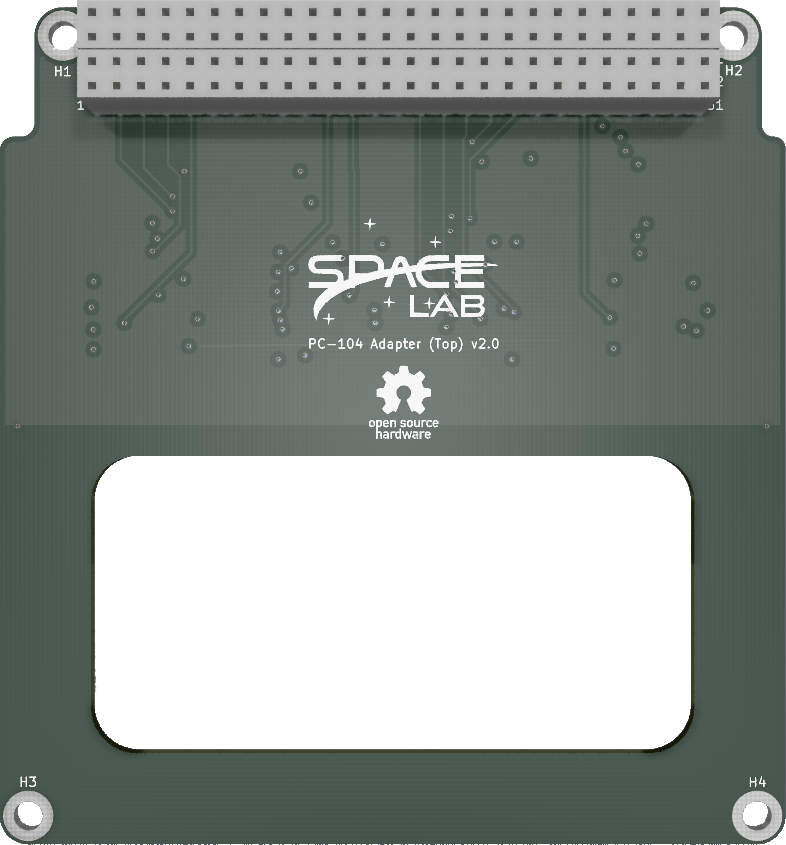
\includegraphics[width=8.636cm]{figures/pc104-adapter-top-top}
        \caption{Top view of the top board (real size).}
        \label{fig:top-board-top}
    \end{center}
\end{figure}

\begin{figure}[!htb]
    \begin{center}
        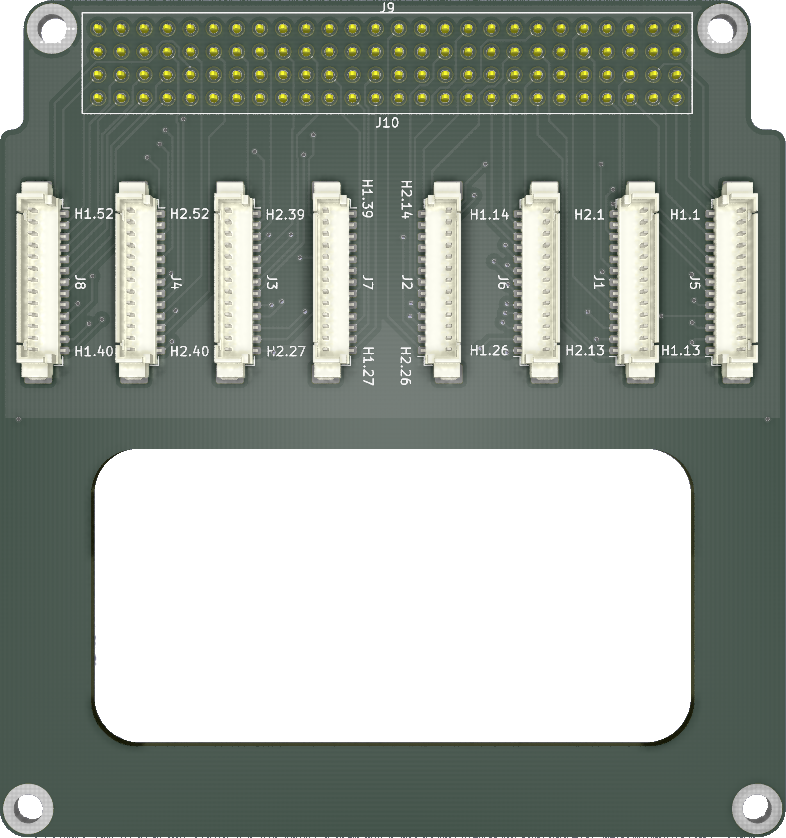
\includegraphics[width=8.636cm]{figures/pc104-adapter-top-bottom}
        \caption{Bottom view of the top board (real size).}
        \label{fig:top-board-bottom}
    \end{center}
\end{figure}

\section{Bottom Board}

The bottom board is composed by eight PicoBlade connectors (13 pins, straight, male) and a male PC-104 connector. A 3D model of the bottom board can be seen in Figures \ref{fig:bottom-board-top} (top side) and \ref{fig:bottom-board-bottom} (bottom side).

\begin{figure}[!htb]
    \begin{center}
        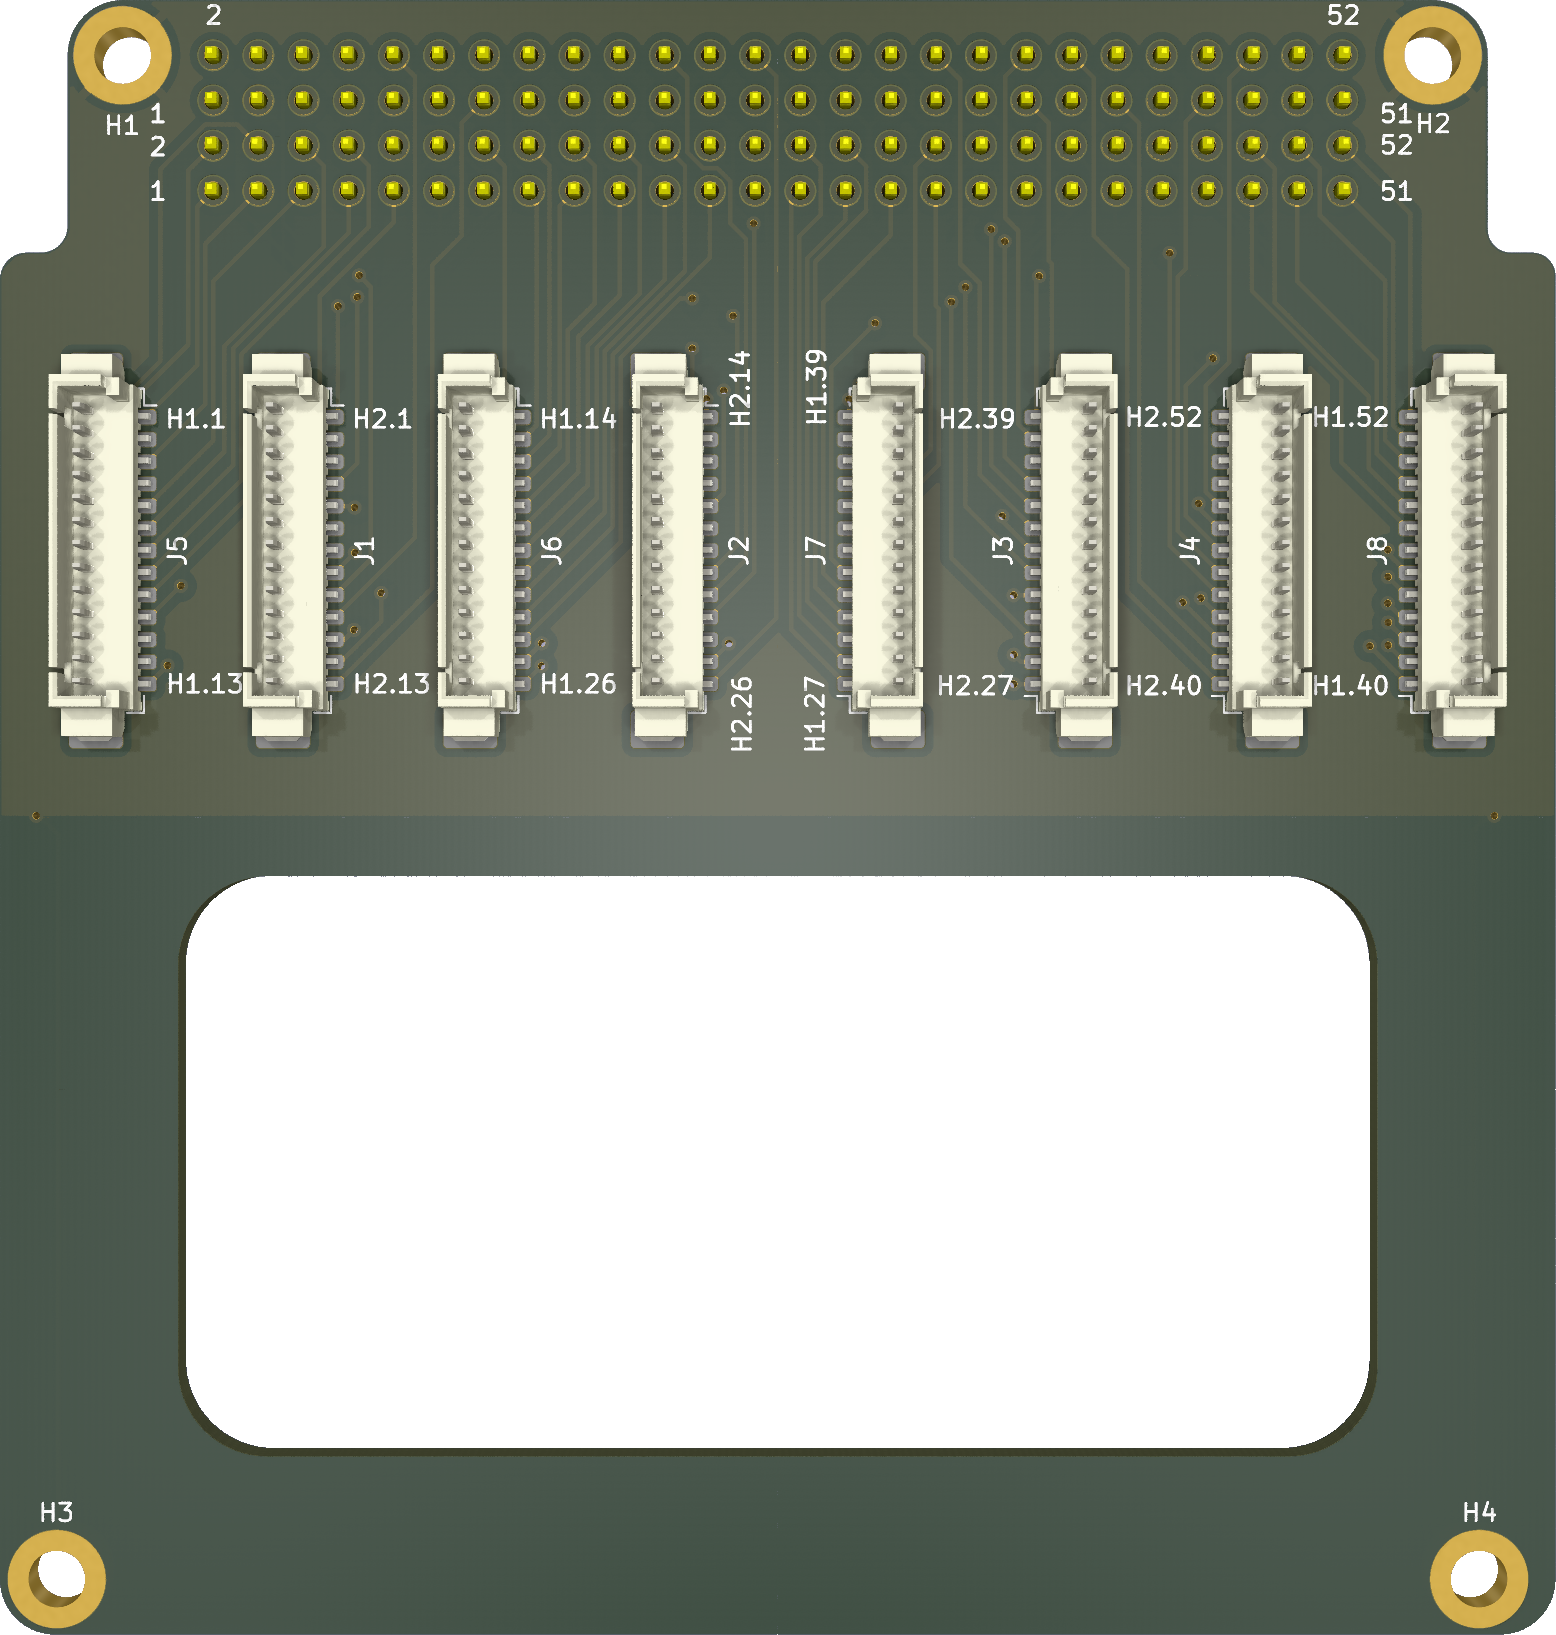
\includegraphics[width=8.626cm]{figures/pc104-adapter-bottom-top}
        \caption{Top view of the bottom board (real size).}
        \label{fig:bottom-board-top}
    \end{center}
\end{figure}

\begin{figure}[!htb]
    \begin{center}
        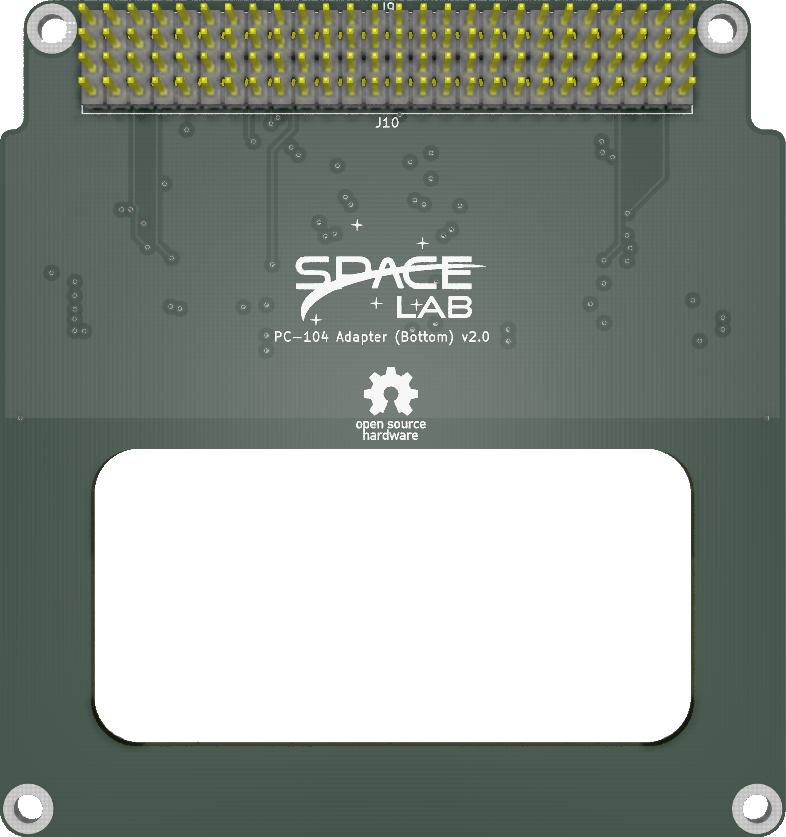
\includegraphics[width=8.626cm]{figures/pc104-adapter-bottom-bottom}
        \caption{Bottom view of the bottom board (real size).}
        \label{fig:bottom-board-bottom}
    \end{center}
\end{figure}

\section{Pinout}

The pinout of the connectors are available in this section. The pin numbering reference of the PC-104 and the PicoBlade connectors can be seen in Figures \ref{fig:pc104-reference} and \ref{fig:picoblade-pin-ref}.

\begin{figure}[!htb]
    \begin{center}
        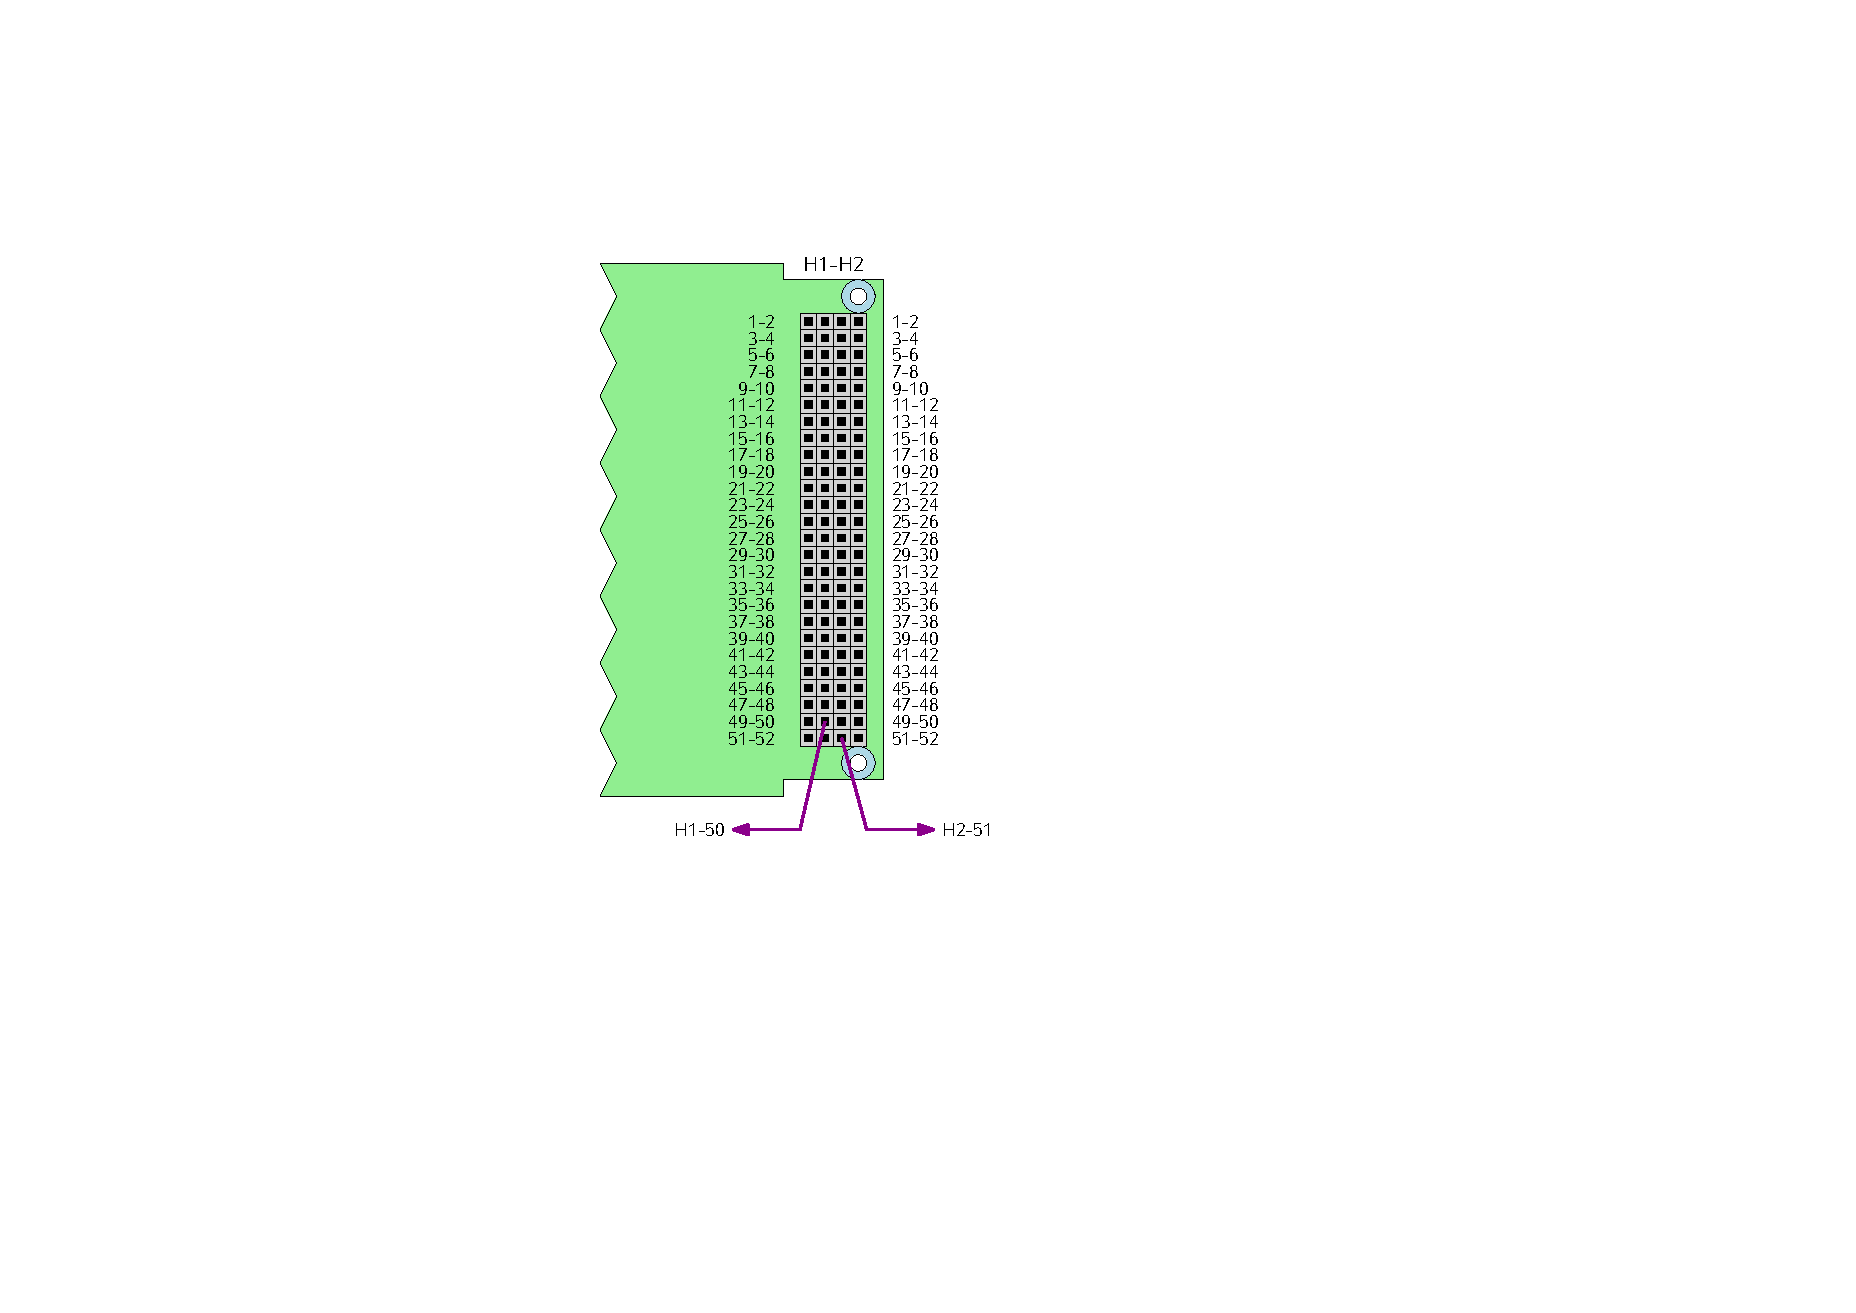
\includegraphics[width=0.45\textwidth]{figures/pc104-diagram}
        \caption{PC-104 pinout reference.}
        \label{fig:pc104-reference}
    \end{center}
\end{figure}

\begin{figure}[!htb]
    \begin{center}
        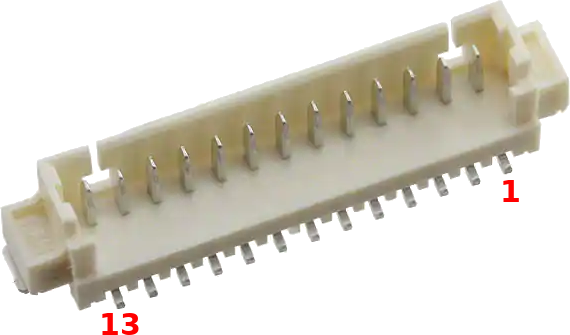
\includegraphics[width=0.5\columnwidth]{figures/picoblade-pin-ref}
        \caption{Pin numbering of the PicoBlade connector.}
        \label{fig:picoblade-pin-ref}
    \end{center}
\end{figure}

The connection between the PicoBlade connectors and the PC-104 bus is available below.

\subsection{Top Board}

In \autoref{tab:pinout-top-board}, the connection between the PicoBlade connectors and the PC-104 bus of the top board is available.

\begin{table}[!h]
    \centering
    \begin{tabular}{crrrrrrrr}
        \toprule[1.5pt]
                               & \multicolumn{8}{c}{\textbf{PC-104 Pin}} \\
        \textbf{PicoBlade Pin} & \textbf{J1} & \textbf{J2} & \textbf{J3} & \textbf{J4} & \textbf{J5} & \textbf{J6} & \textbf{J7} & \textbf{J8} \\
        \midrule
        1                      & H2-13       & H2-26       & H2-39       & H2-52       & H1-13       & H1-26       & H1-39       & H1-52       \\
        2                      & H2-12       & H2-25       & H2-38       & H2-51       & H1-12       & H1-25       & H1-38       & H1-51       \\
        3                      & H2-11       & H2-24       & H2-37       & H2-50       & H1-11       & H1-24       & H1-37       & H1-50       \\
        4                      & H2-10       & H2-23       & H2-36       & H2-49       & H1-10       & H1-23       & H1-36       & H1-49       \\
        5                      & H2-9        & H2-22       & H2-35       & H2-48       & H1-9        & H1-22       & H1-35       & H1-48       \\
        6                      & H2-8        & H2-21       & H2-34       & H2-47       & H1-8        & H1-21       & H1-34       & H1-47       \\
        7                      & H2-7        & H2-20       & H2-33       & H2-46       & H1-7        & H1-20       & H1-33       & H1-46       \\
        8                      & H2-6        & H2-19       & H2-32       & H2-45       & H1-6        & H1-19       & H1-32       & H1-45       \\
        9                      & H2-5        & H2-18       & H2-31       & H2-44       & H1-5        & H1-18       & H1-31       & H1-44       \\
        10                     & H2-4        & H2-17       & H2-30       & H2-43       & H1-4        & H1-17       & H1-30       & H1-43       \\
        11                     & H2-3        & H2-16       & H2-29       & H2-42       & H1-3        & H1-16       & H1-29       & H1-42       \\
        12                     & H2-2        & H2-15       & H2-28       & H2-41       & H1-2        & H1-15       & H1-28       & H1-41       \\
        13                     & H2-1        & H2-14       & H2-27       & H2-40       & H1-1        & H1-14       & H1-27       & H1-40       \\
        \bottomrule[1.5pt]
    \end{tabular}
    \caption{Pinout of the PicoBlade connectors of the Top Board.}
    \label{tab:pinout-top-board}
\end{table}

\subsection{Bottom Board}

In \autoref{tab:pinout-bottom-board}, the connection between the PicoBlade connectors and the PC-104 bus of the bottom board is available.

\begin{table}[!h]
    \centering
    \begin{tabular}{crrrrrrrr}
        \toprule[1.5pt]
                               & \multicolumn{8}{c}{\textbf{PC-104 Pin}} \\
        \textbf{PicoBlade Pin} & \textbf{J1} & \textbf{J2} & \textbf{J3} & \textbf{J4} & \textbf{J5} & \textbf{J6} & \textbf{J7} & \textbf{J8} \\
        \midrule
        1                      & H2-1        & H2-14       & H2-27       & H2-40       & H1-1        & H1-14       & H1-27       & H1-40       \\
        2                      & H2-2        & H2-15       & H2-28       & H2-41       & H1-2        & H1-15       & H1-28       & H1-41       \\
        3                      & H2-3        & H2-16       & H2-29       & H2-42       & H1-3        & H1-16       & H1-29       & H1-42       \\
        4                      & H2-4        & H2-17       & H2-30       & H2-43       & H1-4        & H1-17       & H1-30       & H1-43       \\
        5                      & H2-5        & H2-18       & H2-31       & H2-44       & H1-5        & H1-18       & H1-31       & H1-44       \\
        6                      & H2-6        & H2-19       & H2-32       & H2-45       & H1-6        & H1-19       & H1-32       & H1-45       \\
        7                      & H2-7        & H2-20       & H2-33       & H2-46       & H1-7        & H1-20       & H1-33       & H1-46       \\
        8                      & H2-8        & H2-21       & H2-34       & H2-47       & H1-8        & H1-21       & H1-34       & H1-47       \\
        9                      & H2-9        & H2-22       & H2-35       & H2-48       & H1-9        & H1-22       & H1-35       & H1-48       \\
        10                     & H2-10       & H2-23       & H2-36       & H2-49       & H1-10       & H1-23       & H1-36       & H1-49       \\
        11                     & H2-11       & H2-24       & H2-37       & H2-50       & H1-11       & H1-24       & H1-37       & H1-50       \\
        12                     & H2-12       & H2-25       & H2-38       & H2-51       & H1-12       & H1-25       & H1-38       & H1-51       \\
        13                     & H2-13       & H2-26       & H2-39       & H2-52       & H1-13       & H1-26       & H1-39       & H1-52       \\
        \bottomrule[1.5pt]
    \end{tabular}
    \caption{Pinout of the PicoBlade connectors of the Bottom Board.}
    \label{tab:pinout-bottom-board}
\end{table}

\section{Bill of Materials}

The Bill of Materials (BOM\nomenclature{\textbf{BOM}}{\textit{Bill Of Materials.}}) of the top and bottom boards, and the interconnection cables are available in Tables \ref{tab:bom-top-board}, \ref{tab:bom-bottom-board} and \ref{tab:bom-cables}, respectively.

\begin{table}[!h]
    \centering
    \begin{tabular}{cL{5.8cm}L{5.8cm}r}
        \toprule[1.5pt]
        \textbf{Item}   & \textbf{Designator}            & \textbf{Partnumber} & \textbf{Quantity} \\
        \midrule
        1               & J9, J10                        & SSW-126-01-G-D      & 2                 \\
        2               & J1, J2, J3, J4, J5, J6, J7, J8 & 53398-1371          & 8                 \\
        \bottomrule[1.5pt]
    \end{tabular}
    \caption{Bill of Materials (BOM) of the top board.}
    \label{tab:bom-top-board}
\end{table}

\begin{table}[!h]
    \centering
    \begin{tabular}{cL{5.8cm}L{5.8cm}r}
        \toprule[1.5pt]
        \textbf{Item}   & \textbf{Designator}            & \textbf{Partnumber} & \textbf{Quantity} \\
        \midrule
        1               & J9, J10                        & TSW-126-07-G-D      & 2                 \\
        2               & J1, J2, J3, J4, J5, J6, J7, J8 & 53398-1371          & 8                 \\
        \bottomrule[1.5pt]
    \end{tabular}
    \caption{Bill of Materials (BOM) of the bottom board.}
    \label{tab:bom-bottom-board}
\end{table}

\begin{table}[!h]
    \centering
    \begin{tabular}{cL{5.8cm}L{5.8cm}r}
        \toprule[1.5pt]
        \textbf{Item}   & \textbf{Designator}            & \textbf{Partnumber} & \textbf{Quantity} \\
        \midrule
        1               & -                              & 51021-1300          & 8                 \\
        2               & -                              & 15134-1401          & 16                \\
        \bottomrule[1.5pt]
    \end{tabular}
    \caption{Bill of Materials (BOM) of the connection cables.}
    \label{tab:bom-cables}
\end{table}
